\section{System architecture}
\label{sec:sysarch}

\subsection{Top level}

\begin{figure}
  \centering
  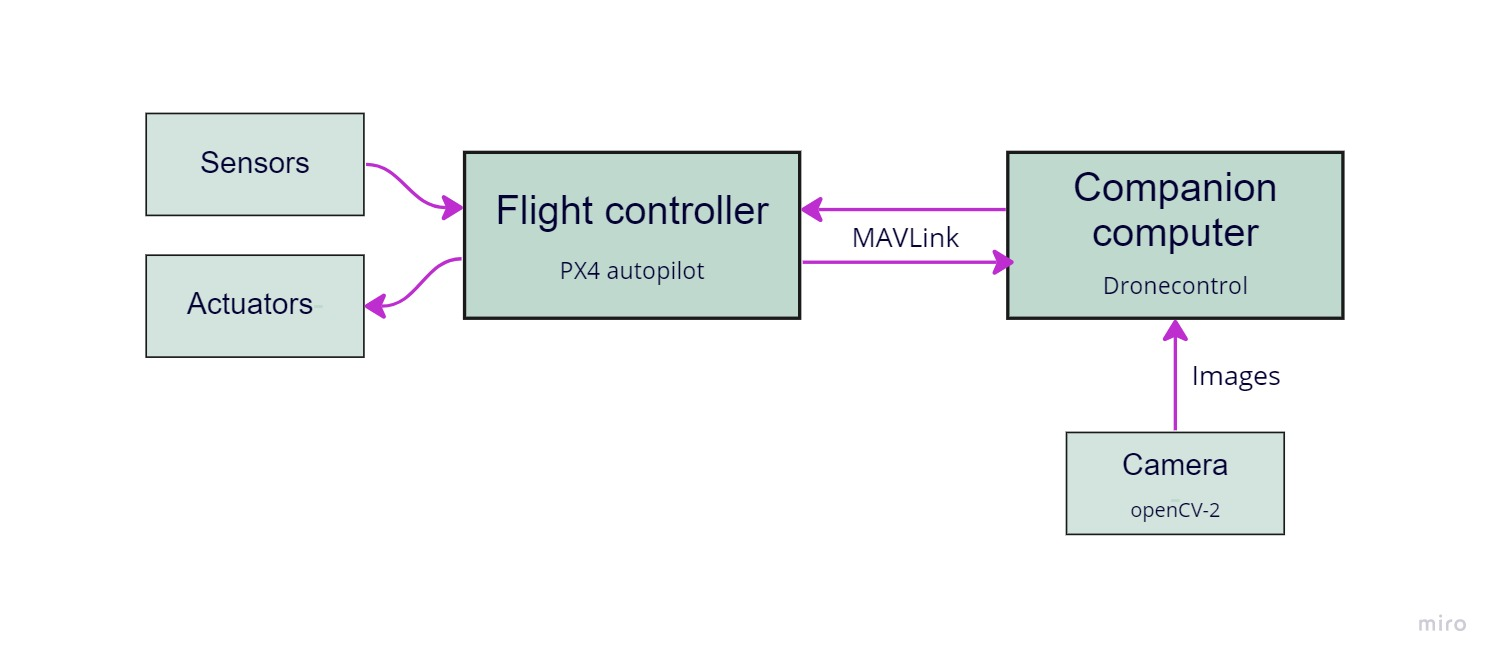
\includegraphics[width=0.9\textwidth,keepaspectratio]{img/sys-arch-diagram.jpg}
  \caption{Top-level diagram of the hardware/software interactions}
  \label{fig:toplevel}
\end{figure}

The purpose of the Dronecontrol application is to be able to direct the movement of a UAV through the analysis of the images taken by a camera.
Since the processing power needed to analyse the images recorded is superior to that offered by the autopilot flight controller, it becomes necessary to use an additional companion computer that can control the camera and leverage machine learning algorithms to extract useful features from the images and transform them into movement directives for the vehicle.

A top-level diagram of the individual parts that comprise the system is shown in figure \ref{fig:toplevel}. The main elements are the flight controller, which will run the PX4 autopilot \ref{subsec:px4}, the companion computer, which will run the developed application, and the camera, which provides the images.
The flight controller interfaces directly with the companion computer using the MAVLink protocol described in section \ref{subsec:mavlink} through a wireless radio link or a cabled serial connection between the two.
The camera is connected to the companion computer through a USB cable into any available port on the computer.
Typically, the type of connection between the flight controller and the computer depends on the system's desired setup.
There are two main possibilities.
When the images have to be taken from the vehicle's perspective and move with it, the camera, and therefore the companion computer, flies onboard the vehicle next to the flight controller. 
In this case, using a direct wire connection between the two is the most convenient, as it provides a faster and more stable link. 
This onboard configuration is detailed in section \ref{subsec:offboard}.
The second possibility is that the companion computer acts more like a ground station, directing the vehicle's movement from the ground on an offboard configuration while the flight controller stays onboard the vehicle.
This configuration is possible when the camera does not need to move with the vehicle.
Then, it becomes strictly necessary to communicate with the flight controller through a wireless connection, using the pair of telemetry radios provided with the Development Kit of the Holybro X500 (\ref{subsec:pixhawk}).
Section \ref{subsec:onboard} describes the complete setup required for this configuration.

In this project, the flight controller is driven by the PX4 flight stack (\ref{subsec:px4}), and the hardware employed on the autopilot board is optimised for this software.
PX4 uses sensors to determine the vehicle state, which is needed for stabilisation and to enable autonomous control.
It minimally requires a gyroscope, accelerometer, magnetometer (compass) and barometer.
A GPS or other positioning system is also needed to activate all fully automatic flight modes, like planned missions, and some assisted ones, like altitude stabilisation.
PX4 uses outputs to control motor speed, flight surfaces like ailerons and flaps, camera triggers, parachutes, grippers, and many other types of payloads.
Most PX4 drones rotate the propellers through brushless motors that the flight controller controls via an Electronic Speed Controller (ESC).
The ESC converts a signal from the flight controller to an appropriate level of power delivered to the motor.
They are most commonly powered by Lithium-Polymer (LiPo) batteries, typically connected to the system using a Power Module or Power Management Board, 
which provides separate power for the flight controller and the ESCs for the motors.
To manually control the vehicle, a Radio Control (RC) system is used.
It consists of a remote control unit that uses a transmitter to communicate stick and control positions to a receiver located on the vehicle.
More complex RC systems can also receive telemetry information from the autopilot to display for the operator.
Other ways of communicating with the autopilot include telemetry radios, which can provide a wireless MAVLink connection between a ground control station and a vehicle running PX4.
This makes it possible to tune parameters while a vehicle is in flight, send flight mode commands, inspect telemetry information or change a mission on the fly.

On an actual UAV, the PX4 software runs on a dedicated piece of hardware like the Pixhawk 4 flight controller described in section \ref{subsec:pixhawk} that includes all the minimal required sensors for flight as well as interfaces to connect additional actuators and I/O systems (RC, telemetry radio).
However, it is also possible to simulate this hardware on a standard Linux computer by building the flight stack from the source code.
This process is described in section (\ref{sec:devenv}).

The Dronecontrol application that runs on the companion computer has been developed using the Python programming language \footnote{\url{https://www.python.org/}}.
It offers good advantages for a project of these characteristics because of its high-level, easy-to-use syntax that usually results in a smaller code base than other comparable languages for small projects, its versatility and its support for object-oriented programming.
Most importantly, Python is widely used with an official package manager called \texttt{pip} that significantly simplifies the use of external libraries and which gathers in its package index \footnote{\url{https://pypi.org/}} thousands of well-tested utilities,
including many machine learning and image processing projects.
Moreover, all the necessary libraries for interacting with PX4 through the MAVLink protocol, object detection and tracking, and simulation (MavSDK, OpenCV, AirSim, Mediapipe) offer a version to use with Python.
As an interpreted language, it can run without complications in any system with Python installed without compiling separate binaries for different operating systems.

The following sections explore deeper into the differences between the two configurations mentioned before: offboard and onboard companion computer.

\subsection{Offboard computer configuration}
\label{subsec:offboard}

The offboard configuration allows the flight controller to communicate and receive orders from a companion computer that is not physically connected to its hardware, so it can stay on the ground while the vehicle flies.
This has the advantage that it allows for a more straightforward configuration without having to be concerned with low-level hardware interactions between the two systems or providing power to the companion computer while in flight.
It also facilitates using a more powerful computer for image processing since there is no need to account for any added weight to the vehicle.
However, the camera remains connected to the computer on the ground, so the images will not be taken from the drone's perspective in flight, which limits the real-world applications of the system.
Other configurations involving a direct connection from a camera to the flight controller and the transmission of its images wirelessly to the companion computer through MAVLink for offboard processing can be feasible with the current technology but fall out of the scope of this project.

In this instance, the wireless link is established through a pair of telemetry radios connecting to a telemetry port on the flight controller and to a USB port in the companion computer.
Since the Pixhawk 4 is configured by default to use its \texttt{TELEM1} port for this purpose, no additional parameter configuration is needed when using that port.
To connect to the board from the companion computer, applications like the QGRoundControl (\ref{subsec:qgc}) ground station software can automatically detect a telemetry radio inserted into any USB port on the host computer.
Additionally, other applications using the MavSDK (\ref{subsec:mavlink}) library can establish a connection by specifying the baudrate and the USB serial port address, usually something similar to \texttt{/dev/ttyUSB0} on Linux and \texttt{COM1} on Windows.

The radio used for the physical tests in this project is the Holybro SiK Telemetry Radio \footnote{\url{http://www.holybro.com/product/transceiver-telemetry-radio-v3/}}.
It is a small, light and inexpensive open-source radio platform that typically allows ranges of more than 300 meters "out of the box" (the range can be extended to several kilometres with a patch antenna on the ground).
The radios are offered as 915Mhz (Europe) or 433Mhz (US), so they can be used in different regions and comply with the regulations for frequency, hopping channels and power levels.
They offer 2-way full-duplex communication through an adaptive TDM UART interface, and their antenna allows for an adjustable 100-mW-maximum output power and -117 dBm receive sensitivity.
The link is established by default with a baudrate (max bits per second on a serial channel) of 57600, and it can provide air data rates of up to 250 kbps.

Figure \ref{fig:offboard-config} summarises the connections to establish between the PX4 software, the Dronecontrol application, their hardware platforms, and their respective peripherals both onboard the vehicle and at the ground station for the offboard computer configuration setup.

\begin{figure}
  \centering
  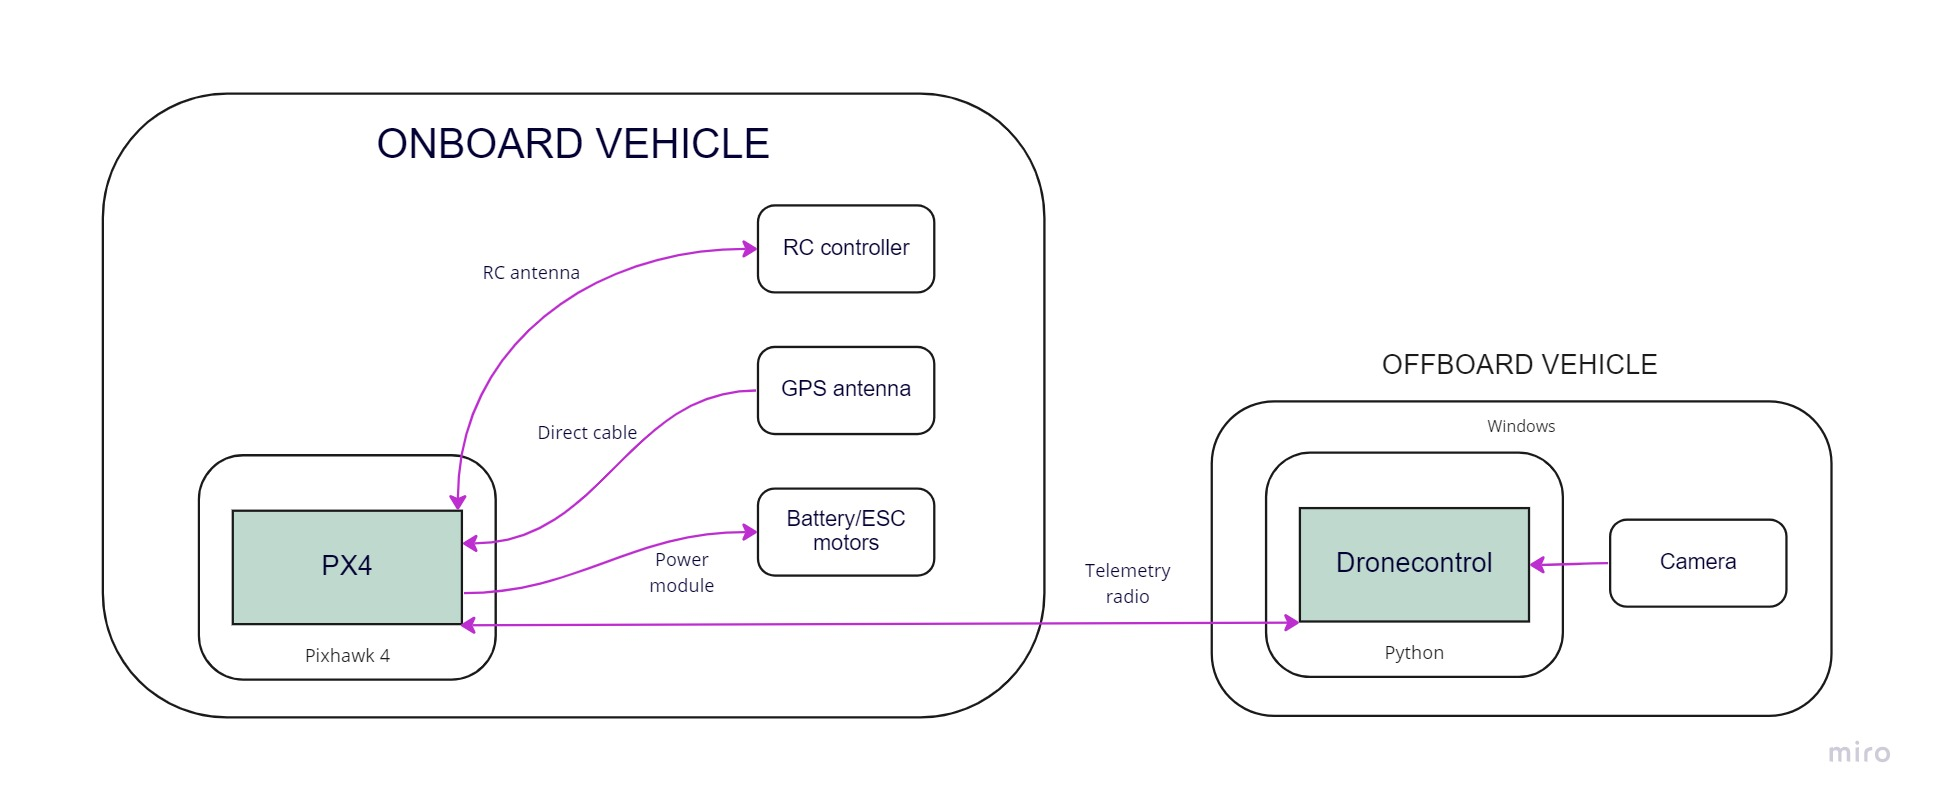
\includegraphics[width=\textwidth,keepaspectratio]{img/offboard-diagram.jpg}
  \caption{Offboard configuration connections}
  \label{fig:offboard-config}
\end{figure}


\subsection{Onboard computer configuration}
\label{subsec:onboard}

The second way of configuring the interaction between the flight controller and the companion computer consists of incorporating both of them together on board the UAV.
In this case, the connection is made through a serial cable between the telemetry port in the flight controller and a serial port in the companion computer.
The camera will then be connected through a cable as well to the companion computer and attached to the frame of the vehicle in a way that allows for a practical perspective during flight.
This configuration makes it possible to develop new control solutions based on images taken directly from the vehicle that reflect the trajectory that it follows.
Therefore, it becomes possible to adjust the control loop based on previous reactions of the vehicle to commands and establish a feedback loop to maintain a stabilised output.

Since, in this configuration, the computer running the visual processing algorithm has to fly on board the vehicle, making a good choice when selecting hardware becomes essential.
To be able to take into the air, the computer has to be light enough that its weight can be lifted by the propellers while maintaining adequate battery autonomy but also powerful enough that the processor can handle the computer vision algorithms required to extract the necessary features from the images taken from the onboard camera that are to be fed to the control loop.

\begin{figure}
  \centering
  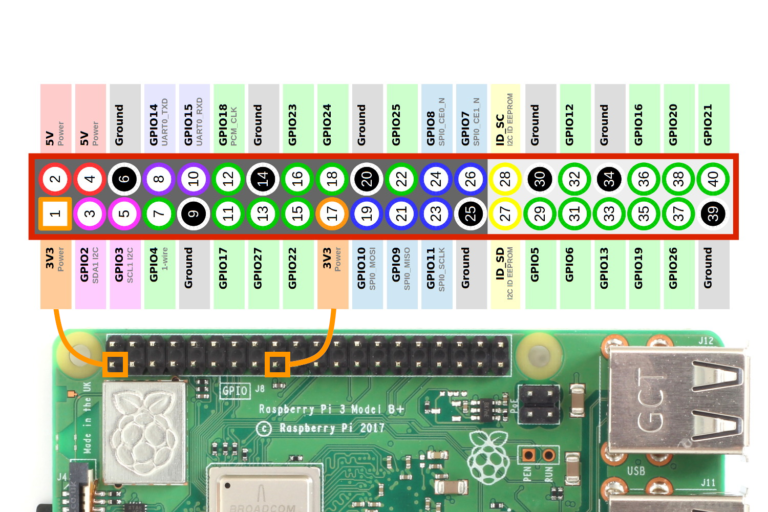
\includegraphics[width=0.8\textwidth,keepaspectratio]{img/rpi4-pinout.png}
  \caption{The Raspberry Pi 4 microcomputer, with its 40-pin GPIO header marked in red and annotated pinout.}
  \source{Adapted from \citetitle{rpi4-pinout} \cite{rpi4-pinout}}
  \label{fig:rpi4-pinout}
\end{figure}

The Raspberry Pi 4 model chosen for this project and shown in figure \ref{fig:rpi4-pinout} is one of the most popular small computers available in the market at the time, and it is widely used in all kinds of robotics projects both for education and hobbyists.
One of the most crucial advantages of using such a platform is the excellent availability of manuals, guides, and other support found on the web.
In addition, the Raspberry's officially supported operating system, called Raspberry Pi OS, is a Debian-based version of Unix optimised for its ARM microcontroller, which simplifies the process of moving from the Ubuntu test environment into the handheld computer.
Since this computer is designed to be easy to integrate with hardware projects, it includes a 40-pin GPIO header (highlighted in figure \ref{fig:rpi4-pinout}) that can be programmed for connecting to any number of external devices.

The Raspberry Pi is powered by a 5V input that can be provided either from its USB-C port or through one of two pins in the header dedicated to this purpose (marked as "5v Power" on figure \ref{fig:rpi4-pinout}).
In the case of the particular vehicle build used in this project, the power management board supplying the energy (the Holybro PM07 \footnote{\url{http://www.holybro.com/product/pixhawk-4-power-module-pm07/}}) also provides 5V to the flight controller, as well as powering the ESCs to the motors.
It counts with two power outputs: one connected to the flight controller's \texttt{POWER1} port and another unused one.
A first attempt at supplying current to the Raspberry Pi from the main battery was tested initially with a connection between the second, free output on the power module and the powering pins on the GPIO header with a custom connector.
However, the consequent power supply ended up being too unstable for the Pi board, resulting in frequent dips in the supplied current that affected the processing capabilities of the companion computer.
The devised solution was to add a secondary battery to the vehicle providing power through a USB to USB-C cable.
This configuration allows the Raspberry to receive power through its default power input, the regulated USB-C port.
The main disadvantage of the solution is that it adds one more piece of equipment of substantial weight that needs to be secured to the vehicle's frame and carried into the air while in flight.

In contrast to the choice of a companion computer, many more possibilities are available regarding the camera that will fly onboard the vehicle.
The most important characteristics to focus on are a small weight and simple plug-and-play functionality with the onboard computer.
The camera used in the tests carried out and detailed in section \ref{chap:validation} is a Logitech C920 1080p webcam \footnote{\url{https://www.logitech.com/es-es/products/webcams/c920-pro-hd-webcam.960-001055.html}}.
Since the frame of the Holybro X500 is not prepared by default to include an onboard camera, a custom mount has been designed and 3D-printed from PLA plastic to be able to hang the camera from the central rods on the underside of the vehicle frame and ensure that it is attached securely during flight.
The 3D model of the mount can be seen in figure \ref{fig:camera-holder-3d}, and the print-ready file can be found in the project repository in GitHub \footnote{\url{https://github.com/l-gonz/tfg-giaa-dronecontrol/blob/main/data/camera-holder.stl}}.

\begin{figure}
  \centering
  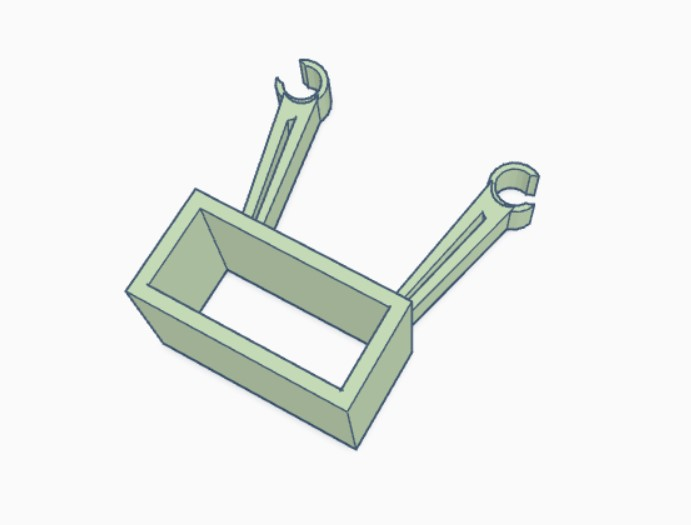
\includegraphics[width=0.6\textwidth, keepaspectratio]{img/cam-holder.jpg}
  \caption{3D model for the camera mount designed for the Holybro X500 frame.}
  \label{fig:camera-holder-3d}
\end{figure}


\begin{figure}
  \centering
  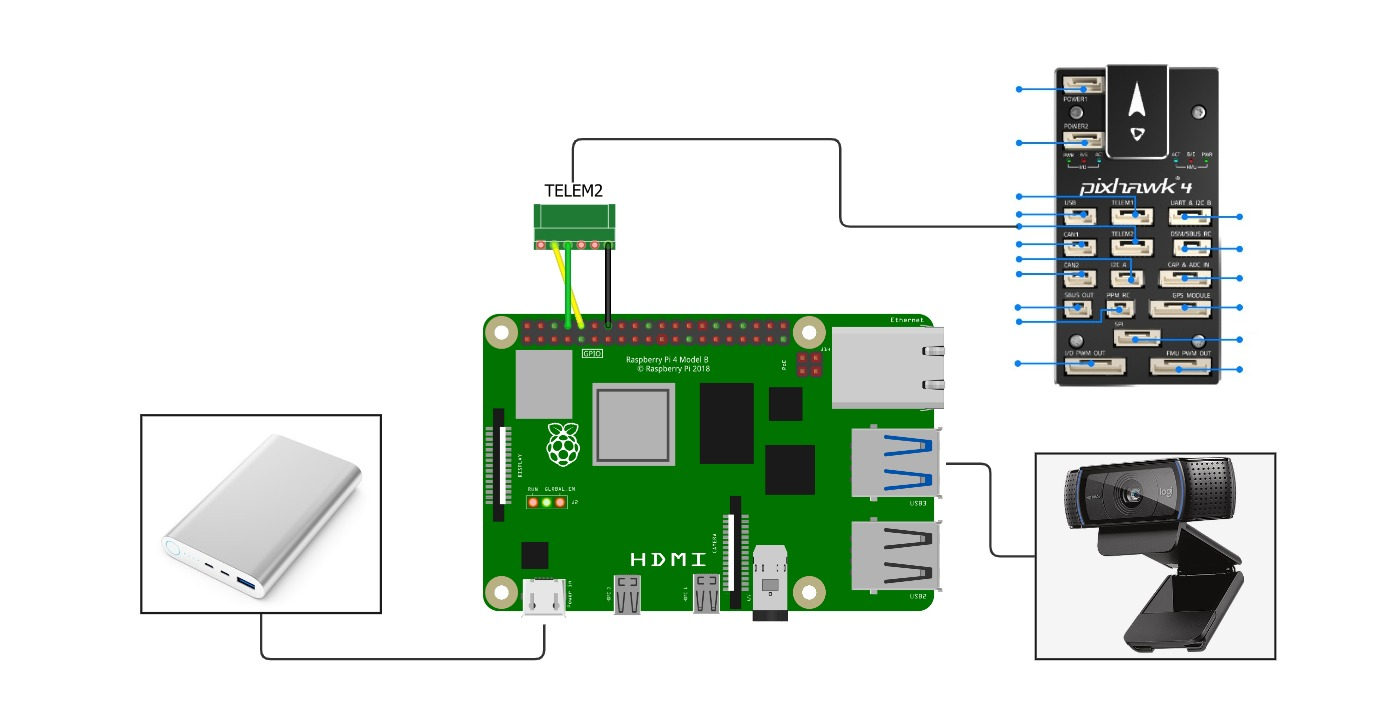
\includegraphics[width=\textwidth,keepaspectratio]{img/wiring-diagram.jpg}
  \caption{A diagram of the wired connections from the Raspberry Pi 4 to the secondary battery and the flight controller (\texttt{TELEM2}).}
  \label{fig:wiring}
\end{figure}


The second wired connection that needs to be established for this configuration is between the flight controller and the companion computer so the MAVLink messages can be exchanged.
As it is desirable to be able to maintain a wireless link to the vehicle even while the onboard computer is controlling it, the telemetry radio is kept connected to the \texttt{TELEM1} port of the flight controller.
Then, the companion computer is wired to the secondary telemetry port, \texttt{TELEM2}.
This port is not configured to be used by default, so it is necessary to modify the configuration of the Pixhawk board either through QGroundControl or the PX4 console to set it up for a companion computer.
The main parameter that requires changing in the board is the \texttt{MAV\_1\_CONFIG}, which configures the serial port on which a second instance of MAVLink is run (the primary instance is configured with \texttt{MAV\_0\_CONFIG}, set up for telemetry radios).
This parameter defaults to 0 (disabled) and should be set to 102 to map to \texttt{TELEM2}.
The secondary MAVLink instance is configured for "Onboard mode" by default, which is the appropriate mode for communicating with a companion computer, instead of the "Normal mode" running on the primary MAVLink instance through \texttt{TELEM1} to communicate with QGroundControl.
Another parameter to consider is the \texttt{SER\_TEL2\_BAUD}, which regulates the baud rate of the \texttt{TELEM2} port.
The default rate is 921600, which is appropriate for a serial connection.
This rate needs to be specified when establishing the connection in the Dronecontrol application through the MAVSDK library.
PX4 provides a complete overview of all the available parameters for the board configuration in their documentation \cite{px4-docs-params}.

The other end of the connector has three female Dupont wires that go into the TX/RX UART pins of the Raspberry Pi,
according to mapping table \ref{tab:wiring-telem} between the six pins in the telemetry connection of the Pixhawk board and the corresponding GPIO pins in the Raspberry Pi header \cite{pixhawk-manual} \cite{pixhawk-px4}.
A diagram of all the connections to the companion computer can be seen in figure \ref{fig:wiring}.

\begin{table}[]
\centering
\begin{tabular}{|ll||ll|}
\hline
\multicolumn{2}{|c||}{\textbf{TELEM2}}                                             & \multicolumn{2}{c|}{\textbf{GPIO header}}                                        \\ \hline \hline
\multicolumn{1}{|c|}{\textit{Pin \#}} & \multicolumn{1}{c||}{\textit{Description}} & \multicolumn{1}{c|}{\textit{Description}} & \multicolumn{1}{c|}{\textit{Pin \#}} \\ \hline
\multicolumn{1}{|l|}{1}               & VCC, +5V                                  & \multicolumn{1}{l|}{}                     &                                      \\ \hline
\multicolumn{1}{|l|}{2}               & TX (out), +3.3V                           & \multicolumn{1}{l|}{GPIO15 (RXD0, UART)}  & 10                                   \\ \hline
\multicolumn{1}{|l|}{3}               & RX (in), +3.3V                            & \multicolumn{1}{l|}{GPIO14 (TXD0, UART)}  & 8                                    \\ \hline
\multicolumn{1}{|l|}{4}               & CTS (in), +3.3V                           & \multicolumn{1}{l|}{}                     &                                      \\ \hline
\multicolumn{1}{|l|}{5}               & RTS (in), +3.3V                           & \multicolumn{1}{l|}{}                     &                                      \\ \hline
\multicolumn{1}{|l|}{6}               & GND                                       & \multicolumn{1}{l|}{GND}                  & 6                                    \\ \hline
\end{tabular}
\caption{Mapping between the \texttt{TELEM2} port in the Pixhawk 4 board and the Raspberry Pi's GPIO header.}
\label{tab:wiring-telem}
\end{table}

Compared to the default baudrate of 57600 on the telemetry radio link established in the previous section, the wired serial connection works at a baudrate of 921600, which means that data can be transferred up to 16 times faster through this link.
However, the main limitation on speed for the program comes from the feature detection process that runs on the images, so a faster link rate will not necessarily mean any increase in the solution's overall performance.
In section \ref{subsec:performance}, different combinations of hardware are compared to analyse any challenges to the program's performance.

The offboard configuration allowed the supervision of the output from the program while the vehicle was flying since the computer stayed stationary on the ground. 
However, having a screen connected directly to the companion computer is not feasible in this configuration.
To fix this situation and be able to monitor the execution during flight, as well as being able to provide input directly to the program, it is possible to make use of the WiFi antenna of the Raspberry Pi to configure a remote desktop and connect to it through another computer serving as a ground station.
Then, the camera output and image recognition can be seen in real-time.

Figure \ref{fig:onboard-config} shows a summary of all the connections present in the onboard configuration between the three pieces of software that interact together: PX4, Dronecontrol and QGroundControl, with their respective hardware platforms and the attached peripherals.

\begin{figure}
  \centering
  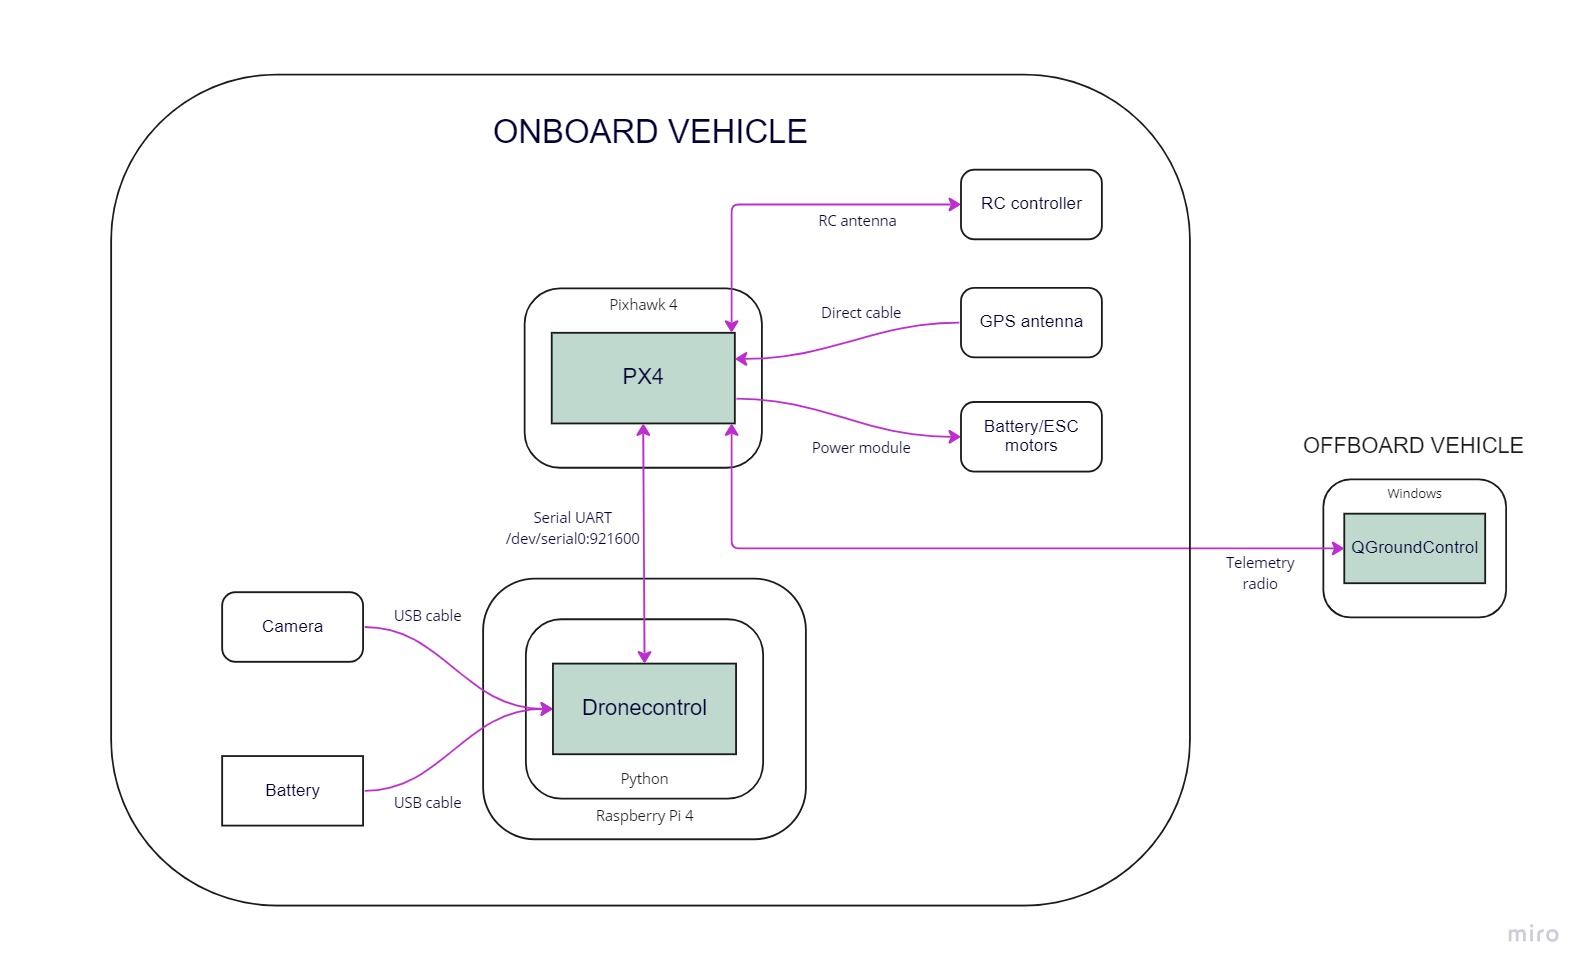
\includegraphics[width=\textwidth,keepaspectratio]{img/onboard-diagram.jpg}
  \caption{Onboard configuration connections}
  \label{fig:onboard-config}
\end{figure}
